\section{A CNDP-től a BOCNDP-ig}

Az egycélú CNDP-től úgy jutunk el a kétcélú CNDP-ig, hogy ebben az esetben két függvényt fogunk optimalizálni.
Míg a CNDP esetén \aref{eqn:PAIRWISE_CONNECTIVITY} képlettel leírt függvény minimalizálása volt a feladat,
addig a BOCNDP esetén két célfüggvényünk van, amelyeket optimalizálni szeretnénk $k$ csomópont kitörlése után a $G$ gráfból:
\begin{enumerate}
  \item Maximalizálni szeretnénk az összefüggő komponensek számát.
  \item Minimalizálni szeretnénk az összefüggő komponensek számosságának a varianciáját.
\end{enumerate}

Ennek érdekében a következő két célfüggvényt vezetjük be:
\begin{equation}\label{eqn:MAX_CONNECTED_COMPONENTS}
  \max \quad \abs{H},
\end{equation}
\begin{equation}\label{eqn:MIN_CARDINALITY_VARIANCE_COMPONENTS}
  \min \quad var(H),
\end{equation}
ahol $H$-val jelöljük a $G\left[ V \setminus S \right]$ feszített részgráf összefüggő komponenseinek a halmazát,
és $var(H)$ jelöli az összefüggő komponensek számosságának nem szabályos mintavételének a varianciáját.
A H halmaz varianciáját a következő képlet segítségével számoljuk ki:
\begin{equation}\label{eqn:CARDINALITY_VARIANCE_COMPONENTS}
  \dfrac{1}{ \abs{H} } \sum_{h \in H} \left( \abs{h} - \dfrac{ n^{*} }{ \abs{H} } \right)^{2},
\end{equation}
ahol $n^{*} = \sum_{h \in H} \abs{h}$ a $G\left[ V \setminus S \right]$ feszített részgráf csomópontjainak a száma.

\Aref{eqn:MAX_CONNECTED_COMPONENTS} és \aref{eqn:CARDINALITY_VARIANCE_COMPONENTS}
képletekkel leírt problémát úgy ismerjük az irodalomban \cite{ventresca2018bi}, mint \textbf{BOCNDP}.
A CNDP is ugyanerre a problémára nyújt megoldást azáltal,
hogy ezt a két függvényt egyesíti \aref{eqn:PAIRWISE_CONNECTIVITY} függvényben,
melynek minimalizálása (lásd \aref{eqn:MIN_PAIRWISE_CONNECTIVITY} egyenlet) maximalizálni fogja a komponensek számát, amelyekre szétesik az eredeti gráf,
de ugyanakkor minimalizálja is a komponensek közötti varianciát.

A $H$ halmaz számosságának meghatározását \aref{lst:NO-CONNECTED-COMPONENTS}. kódrészlet mutatja be Python-ban,
míg \aref{eqn:CARDINALITY_VARIANCE_COMPONENTS} képlet implementációját \aref{lst:CARDINALITY-VARIANCE-COMPONENTS}. kódrészlet.

\lstinputlisting[
  language={Python},
  caption={A feszített részgráf összefüggő komponenseinek a száma},
  label={lst:NO-CONNECTED-COMPONENTS}
]{./progfiles/bi-objective-cndp/no_connected_components.py}

\lstinputlisting[
  language={Python},
  caption={Az összefüggő komponensek számosságának a varianciája},
  label={lst:CARDINALITY-VARIANCE-COMPONENTS}
]{progfiles/bi-objective-cndp/cardinality_variance_components.py}


\subsubsection{Egy példa}
\Aref{fig:BOCNDP_EXAMPLE} ábrán látható gráfban, ha $k = 2$ kritikus csomópontot kell azonosítanunk,
akkor $S = \left\{ 2, 3 \right\}$ eredményezi az optimális megoldást.
A $G\left[ V \setminus S \right]$ feszített részgráf szétesik egy egy csomópontból álló,
és négy három csomópontból álló komponensre, vagyis $\abs{H} = 5$.
Így \aref{eqn:CARDINALITY_VARIANCE_COMPONENTS} képlettel leírt komponensek közötti variancia a következőképpen számolható ki:
\[
  var(H) = \dfrac{1}{5} \cdot \left[ \left( 1 - \dfrac{13}{5} \right)^{2} + 4 \cdot \left( 3 - \dfrac{13}{5} \right)^{2} \right] = \dfrac{16}{25} = 0.64.
\]


\begin{figure}[t]
  \centering
  \begin{tabular}{ll}
    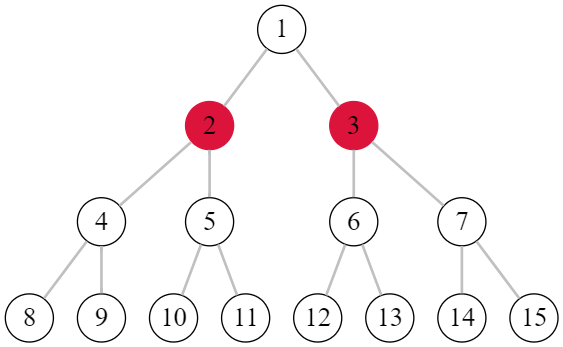
\includegraphics[scale=0.38]{images/bocndp_before.png}
     &
    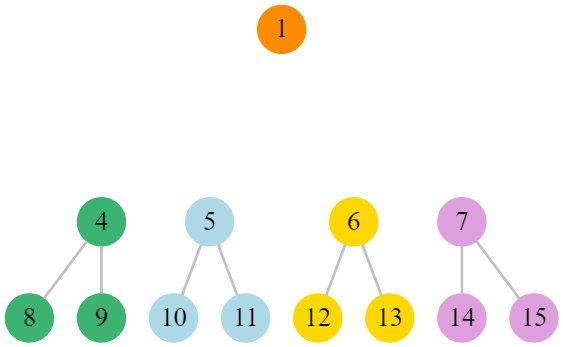
\includegraphics[scale=0.38]{images/bocndp_after.png}
  \end{tabular}
  \caption{
    Példa egy kis méretű gráfra (bal oldalt), amely a 2. és 3. csomópontok (piros színnel emeltük ki ezeket) törlése után
    szétesik öt összefüggő komponensre (jobb oldalt), amelyeket különböző színekkel jelöltünk meg a könnyebb láthatóság kedvéért.
  }
  \label{fig:BOCNDP_EXAMPLE}
\end{figure}
